%%%%%%%%%%%%%%%%%%%%%%%%%%%%%%%%%%%%%%%%%%%%%%%%%%%%%%%%%%%%%%%
\subsection{Vertexing}

%%%%%%%%%%%%%%%%%%%%%%%%%%%%%%%%%%%%%%%%%%%%%%%%%%%%%%%%%%%%%%%
\subsection{Tracking}

\fix{Tracking Efficiency plots need to be redone with pair-bg overlaid !}

%
% tracking resolution for single muons
% 
\thisfloatsetup{floatwidth=\SfigwFull,capposition=beside}
\begin{figure}[b!]
\begin{tabular}{cc}
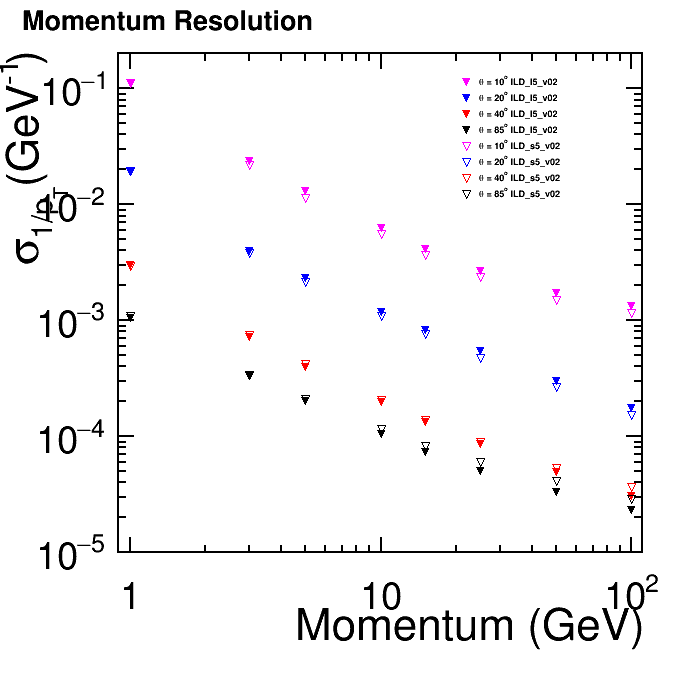
\includegraphics[width=0.5\hsize]{Performance/fig/PResolution_ILD_ls5_v02.png} &
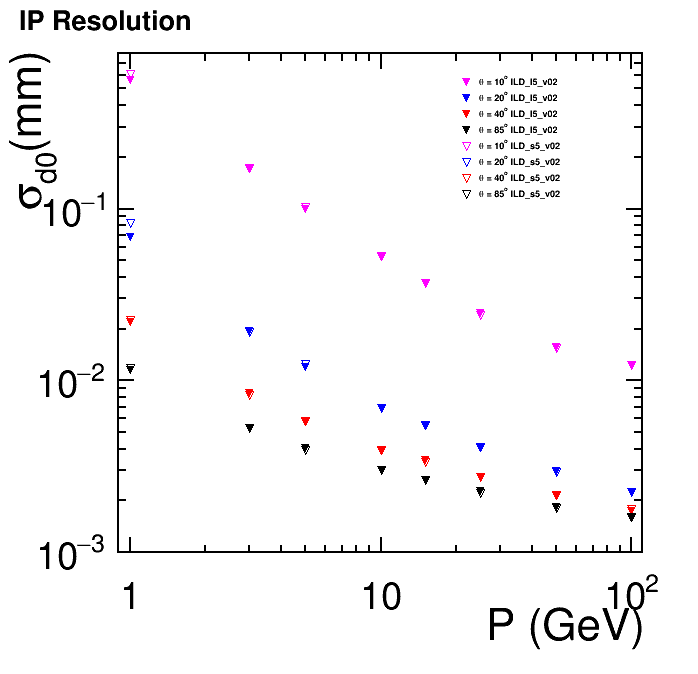
\includegraphics[width=0.5\hsize]{Performance/fig/IPResolution_ILD_ls5_v02.png}
\end{tabular}
\caption{\label{fig:perf:trkres} Momentum (left) and impact parameter (right) resolution for the two ILD detector models,
  as a function of momentum of the single muon. Large detector: closed symbols - small detector: open symbols.}
\end{figure}


%
% tracking efficiency for ttbar - 1D
% 
\thisfloatsetup{floatwidth=\SfigwFull,capposition=beside}
\begin{figure}[b!]
\begin{tabular}{cc}
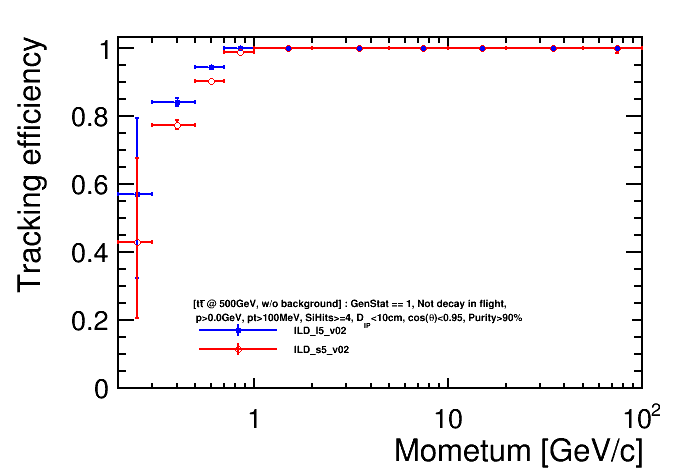
\includegraphics[width=0.5\hsize]{{Performance/fig/trkEff_Momentum_ttbar_ILD_ls5_v02_publish2}.png} &
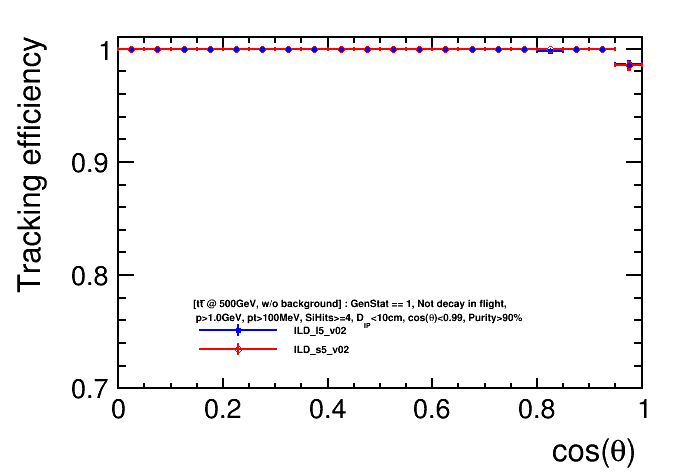
\includegraphics[width=0.5\hsize]{{Performance/fig/trkEff_theta_ttbar_ILD_ls5_v02_publish1}.png}
\end{tabular}
\caption{\label{fig:perf:trkeff_p}Track finding efficiency for $t \bar t$-events at 500 GeV, as a function of momentum (left) and 
 $cos(\theta)$ (right) for the large (red) and small (blue) ILD detector models. }
\end{figure}


%
% tracking efficiency for ttbar - as function of pt
% 
\thisfloatsetup{floatwidth=\SfigwFull,capposition=beside}
\begin{figure}[b!]
\begin{tabular}{cc}
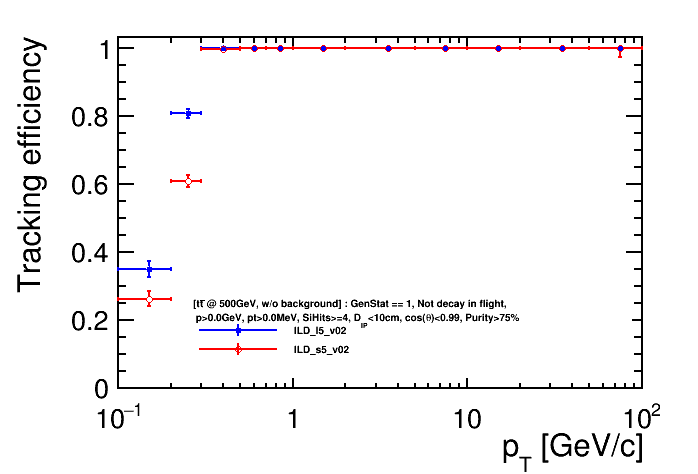
\includegraphics[width=0.5\hsize]{{Performance/fig/trkEff_pt_ttbar_ILD_ls5_v02_monitor}.png} &
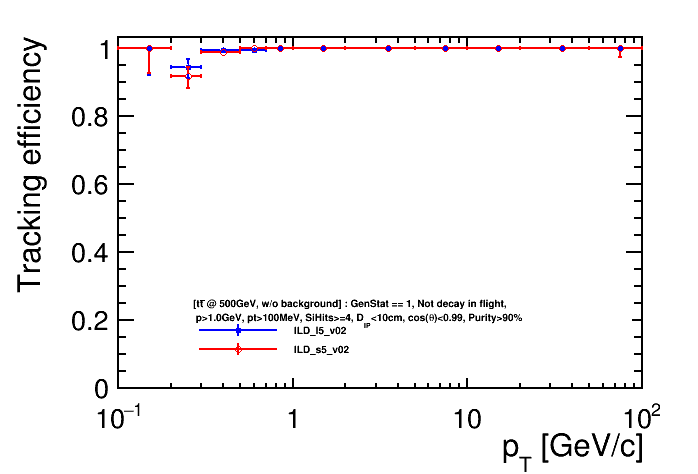
\includegraphics[width=0.5\hsize]{{Performance/fig/trkEff_pt_ttbar_ILD_ls5_v02_publish1}.png}
\end{tabular}
\caption{\label{fig:perf:trkeff_pt}Track finding efficiency for $t \bar t$-events at 500 GeV, as a function of transeverse momentum for the large (red)
  and small (blue) ILD detector models. left: $p > 0$~GeV ; right: $p > 1$~GeV }
\end{figure}


%
% tracking efficiency for ttbar - 2D
% 
\thisfloatsetup{floatwidth=\SfigwFull,capposition=beside}
\begin{figure}[b!]
\begin{tabular}{cc}
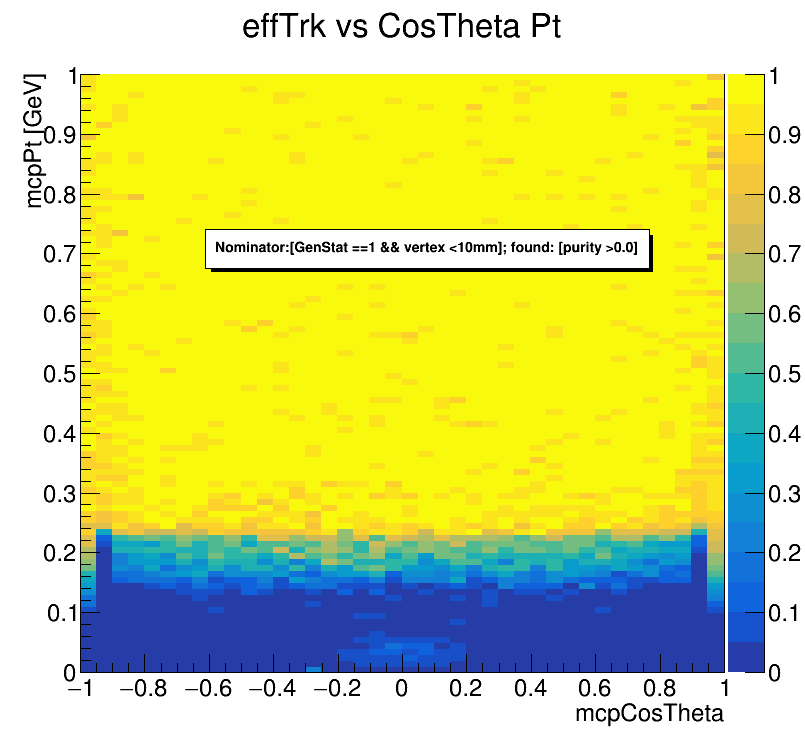
\includegraphics[width=0.5\hsize]{{Performance/fig/EffTrkPerformance2DcosThetaPt_purity0.0}.png} &
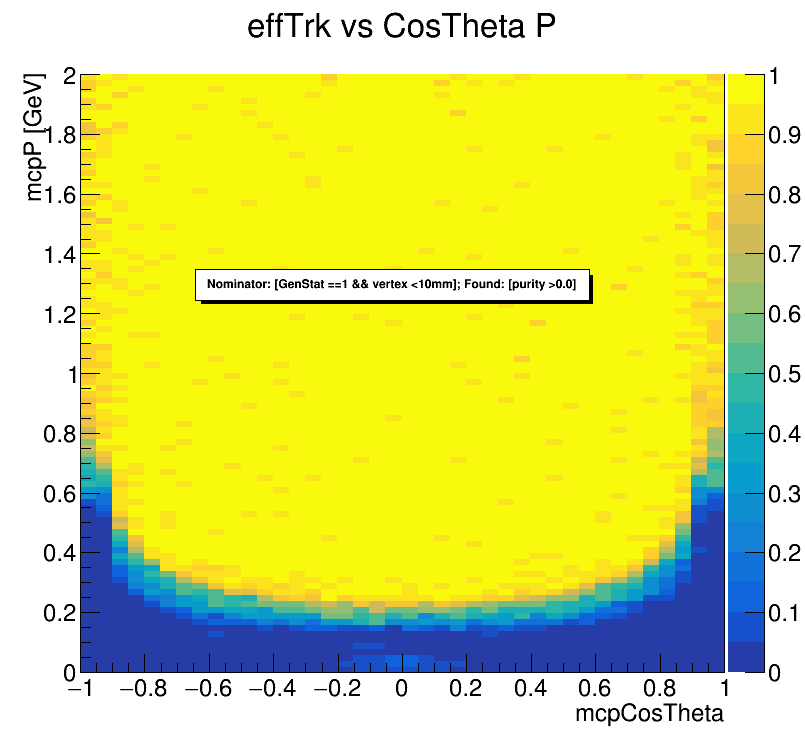
\includegraphics[width=0.5\hsize]{{Performance/fig/EffTrkPerformance2DcosThetaMomentum_purity0.0}.png}
\end{tabular}
\caption{\label{fig:perf:trkeff_2D}Track finding efficiency for $t \bar t$-events at 500 GeV, as a function of transverse momentum (left),
  momentum (right) and $cos(\theta)$ for the large ILD detector model. }
\end{figure}



%
% tracking efficiency for single muons - 2D
% 
\thisfloatsetup{floatwidth=\SfigwFull,capposition=beside}
\begin{figure}[b!]
\begin{tabular}{cc}
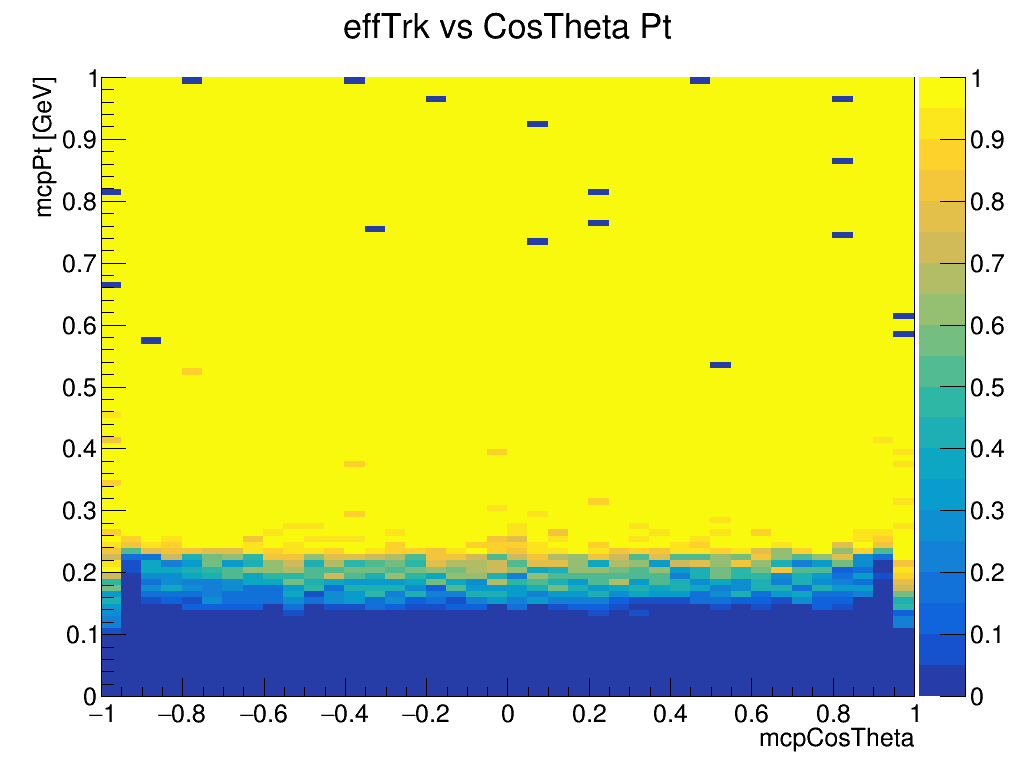
\includegraphics[width=0.5\hsize]{Performance/fig/SingleMuon_EffTrk2DCosThetaPt.png} &
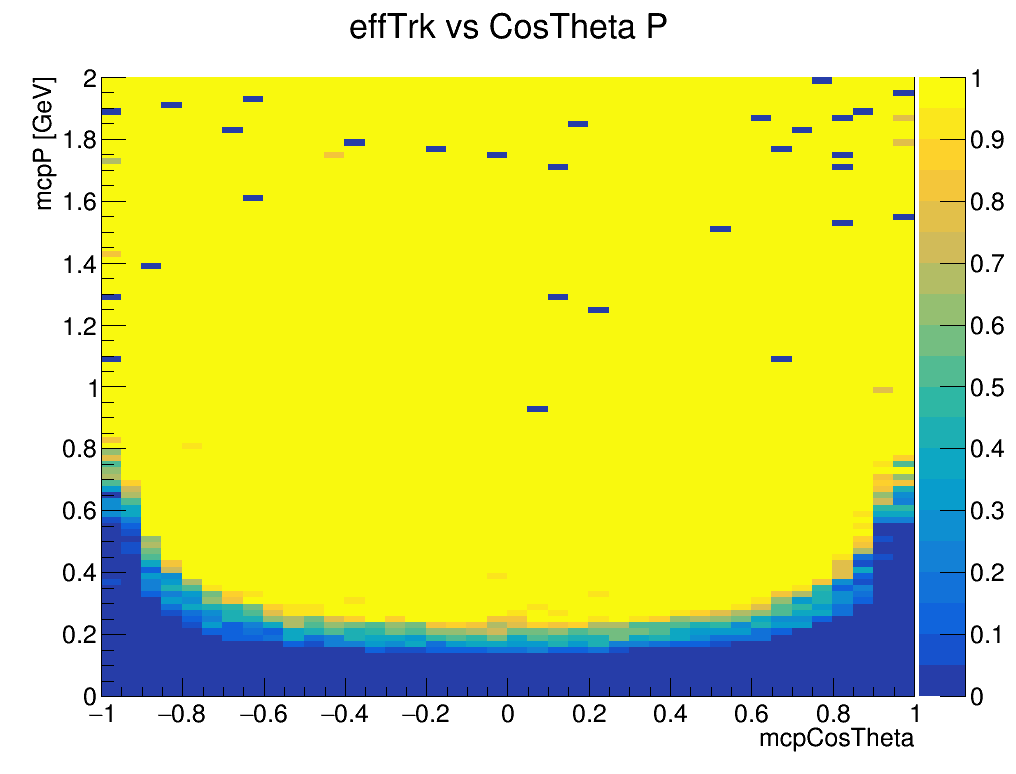
\includegraphics[width=0.5\hsize]{Performance/fig/SingleMuon_EffTrk2DCosThetaP.png}
\end{tabular}
\caption{\label{fig:perf:trkeff_2D_single}Track finding efficiency for single muons as a function of transverse momentum (left),
  momentum (right) and $cos(\theta)$ for the large ILD detector model. \fix{FG: do we need these single particle eff. plots ?} }
 \end{figure}


%%%%%%%%%%%%%%%%%%%%%%%%%%%%%%%%%%%%%%%%%%%%%%%%%%%%%%%%%%%%%%%
\subsection{Particle Flow performance and JER}


%
% uds - JER w/ rms90 and JES
% 
\thisfloatsetup{floatwidth=\SfigwFull,capposition=beside}
\begin{figure}[b!]
\begin{tabular}{cc}
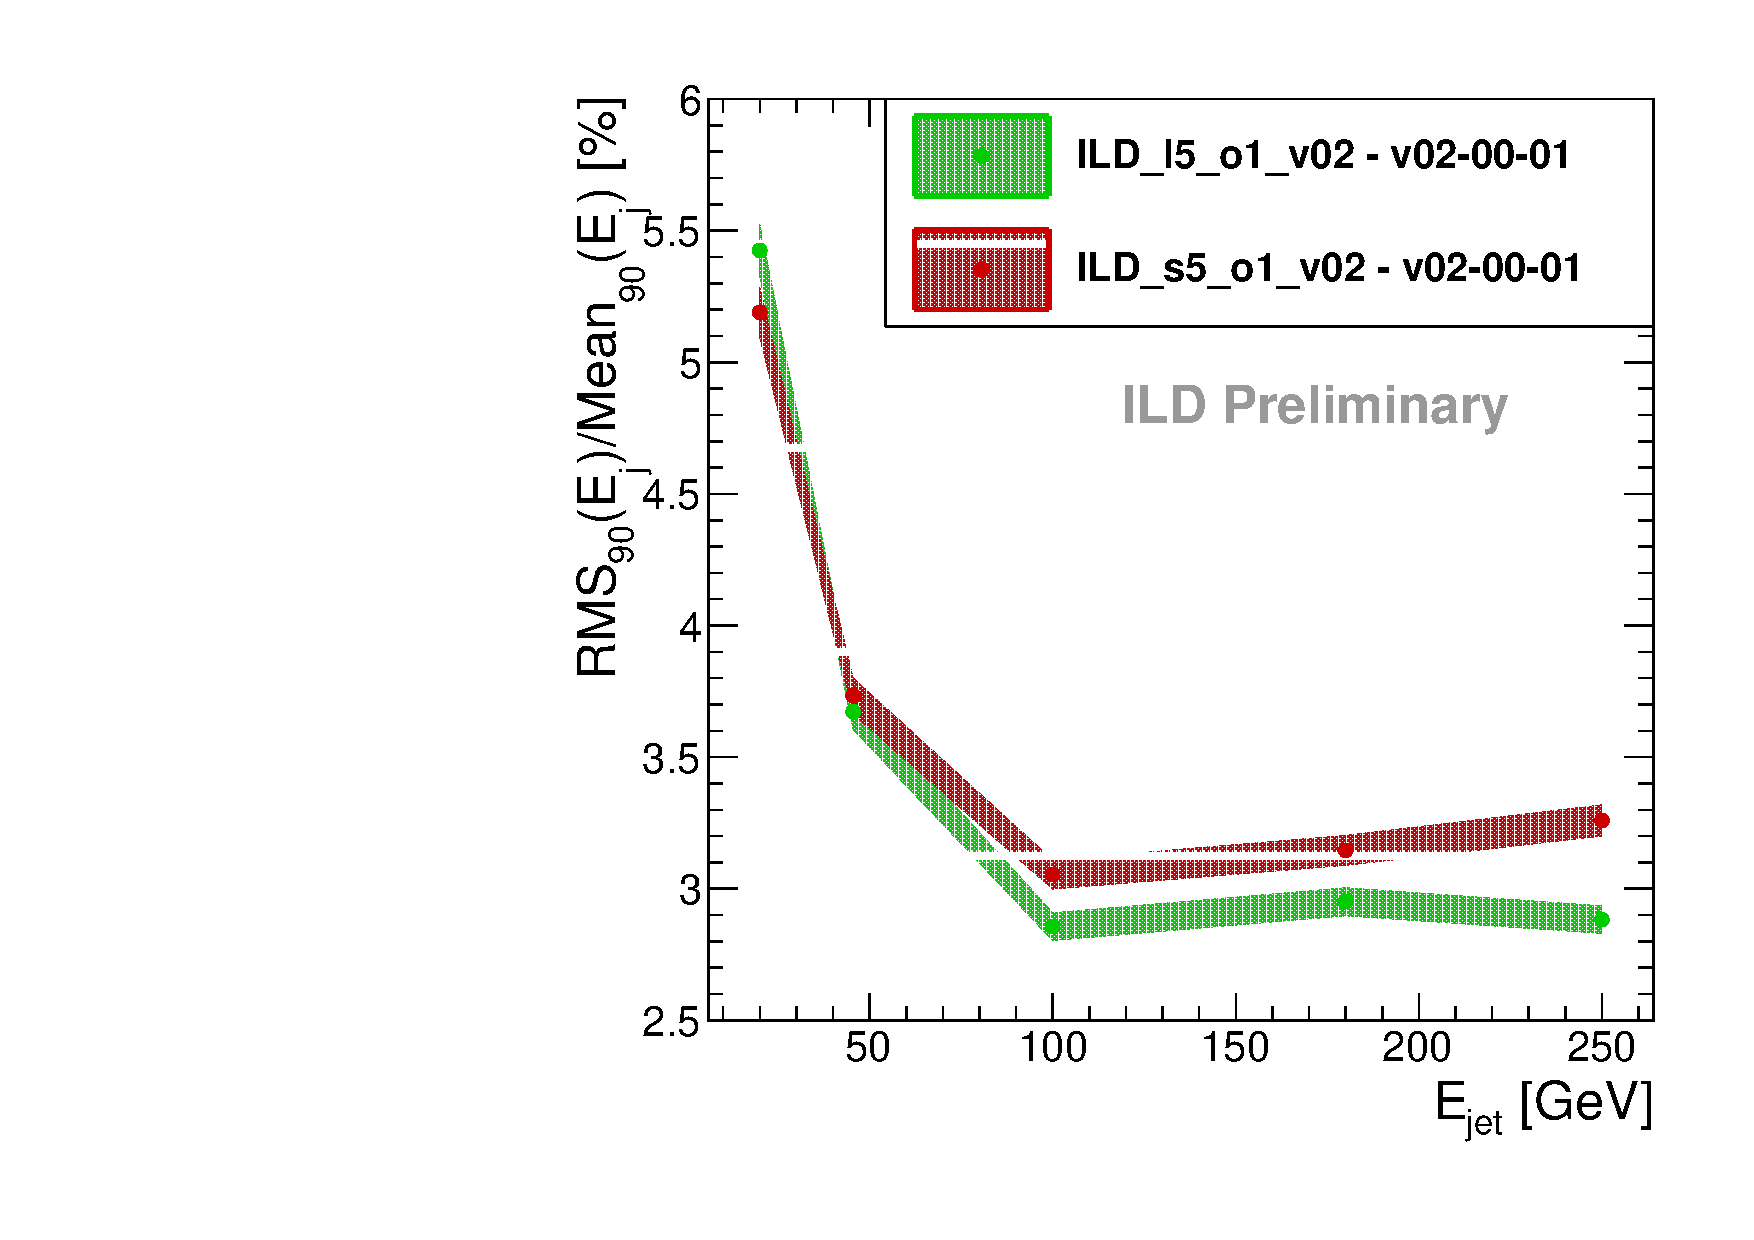
\includegraphics[width=0.5\hsize]{Performance/fig/JERLargeSmall_v02-00-01.pdf} &
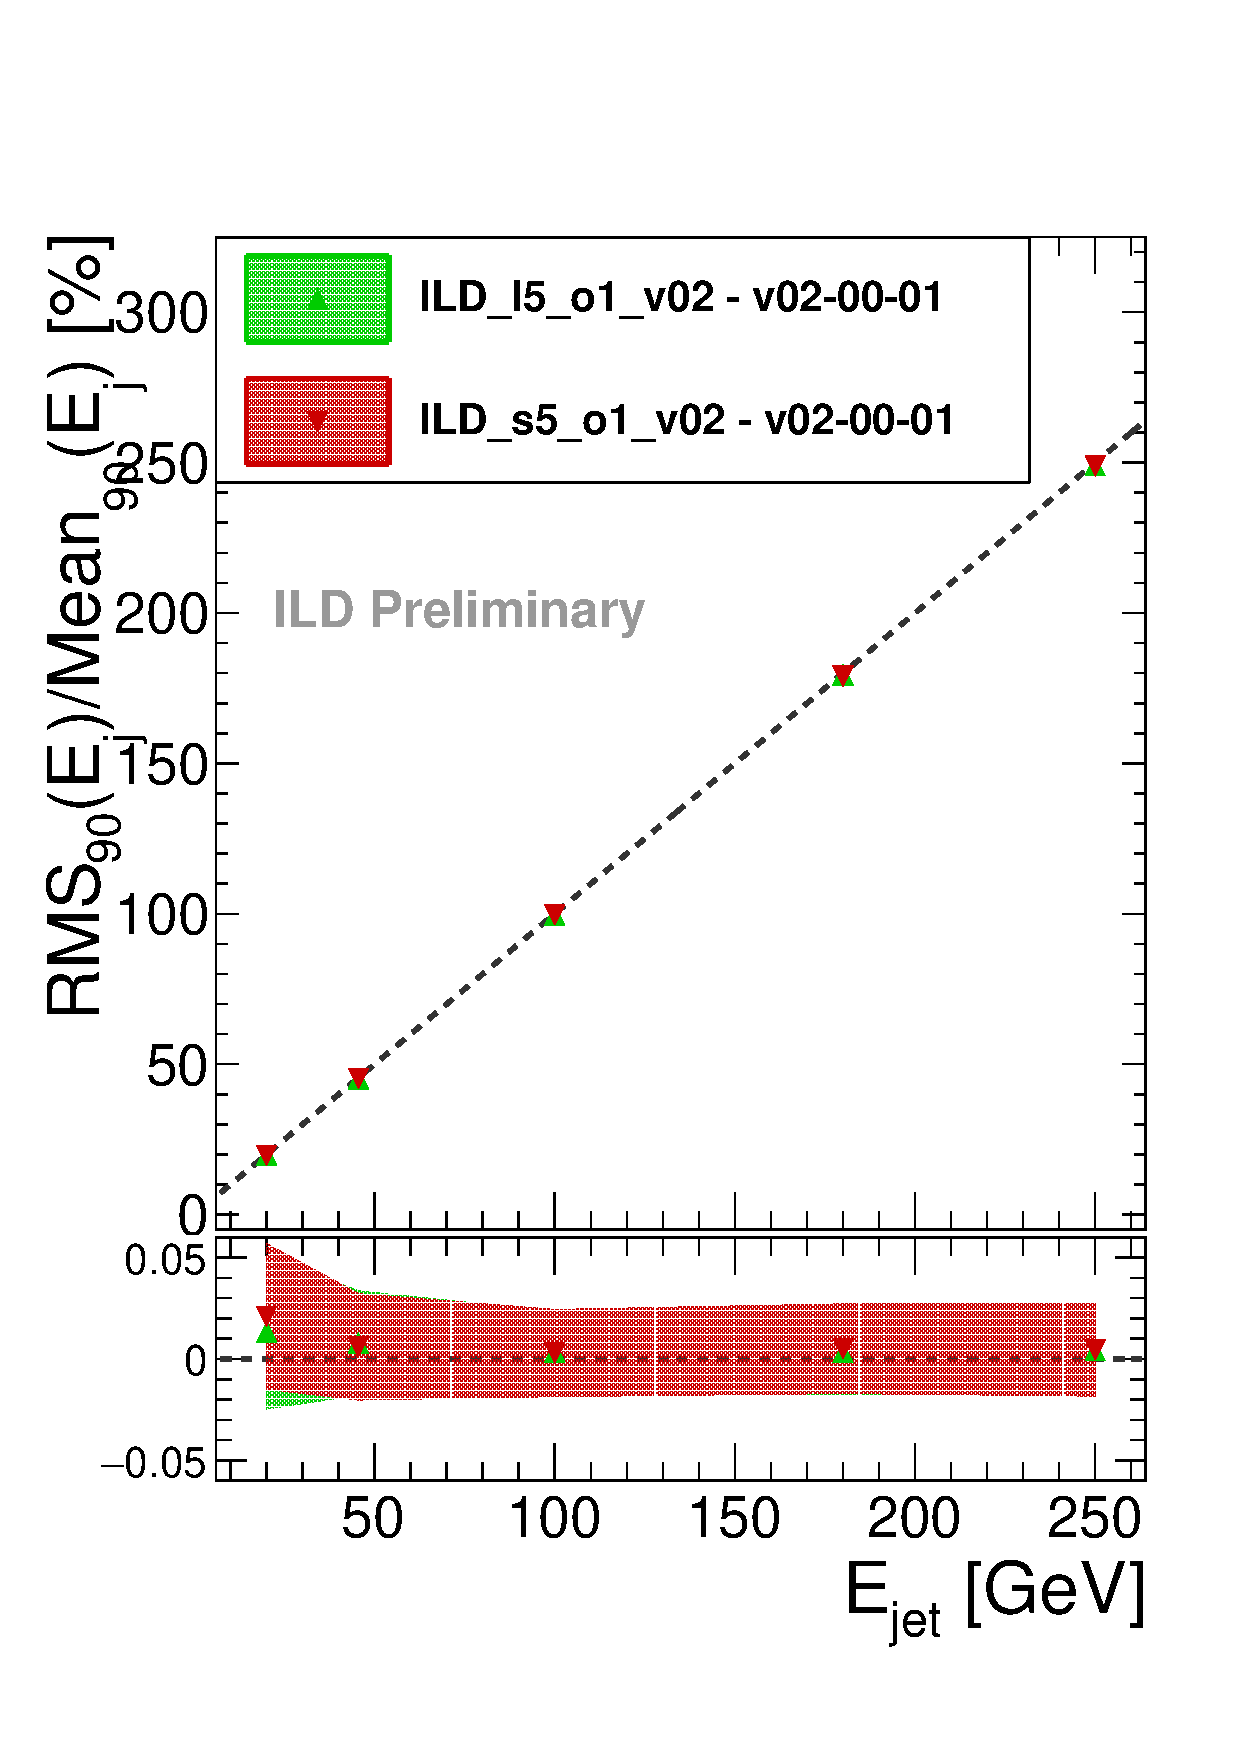
\includegraphics[width=0.5\hsize]{Performance/fig/JESLargeSmall_v02-00-01.pdf}
\end{tabular}
\caption{\label{fig:perf:trkeff_jer_ls} Jet energy resolution (left) and jet energy scale (right) for the large and small ILD detector
models as a function of the jet energy for uds di-jet events.}
 \end{figure}


%
% uds and bb/cc- JER w/ rms90 and JES - large ILD
% 
\thisfloatsetup{floatwidth=\SfigwFull,capposition=beside}
\begin{figure}[b!]
\begin{tabular}{cc}
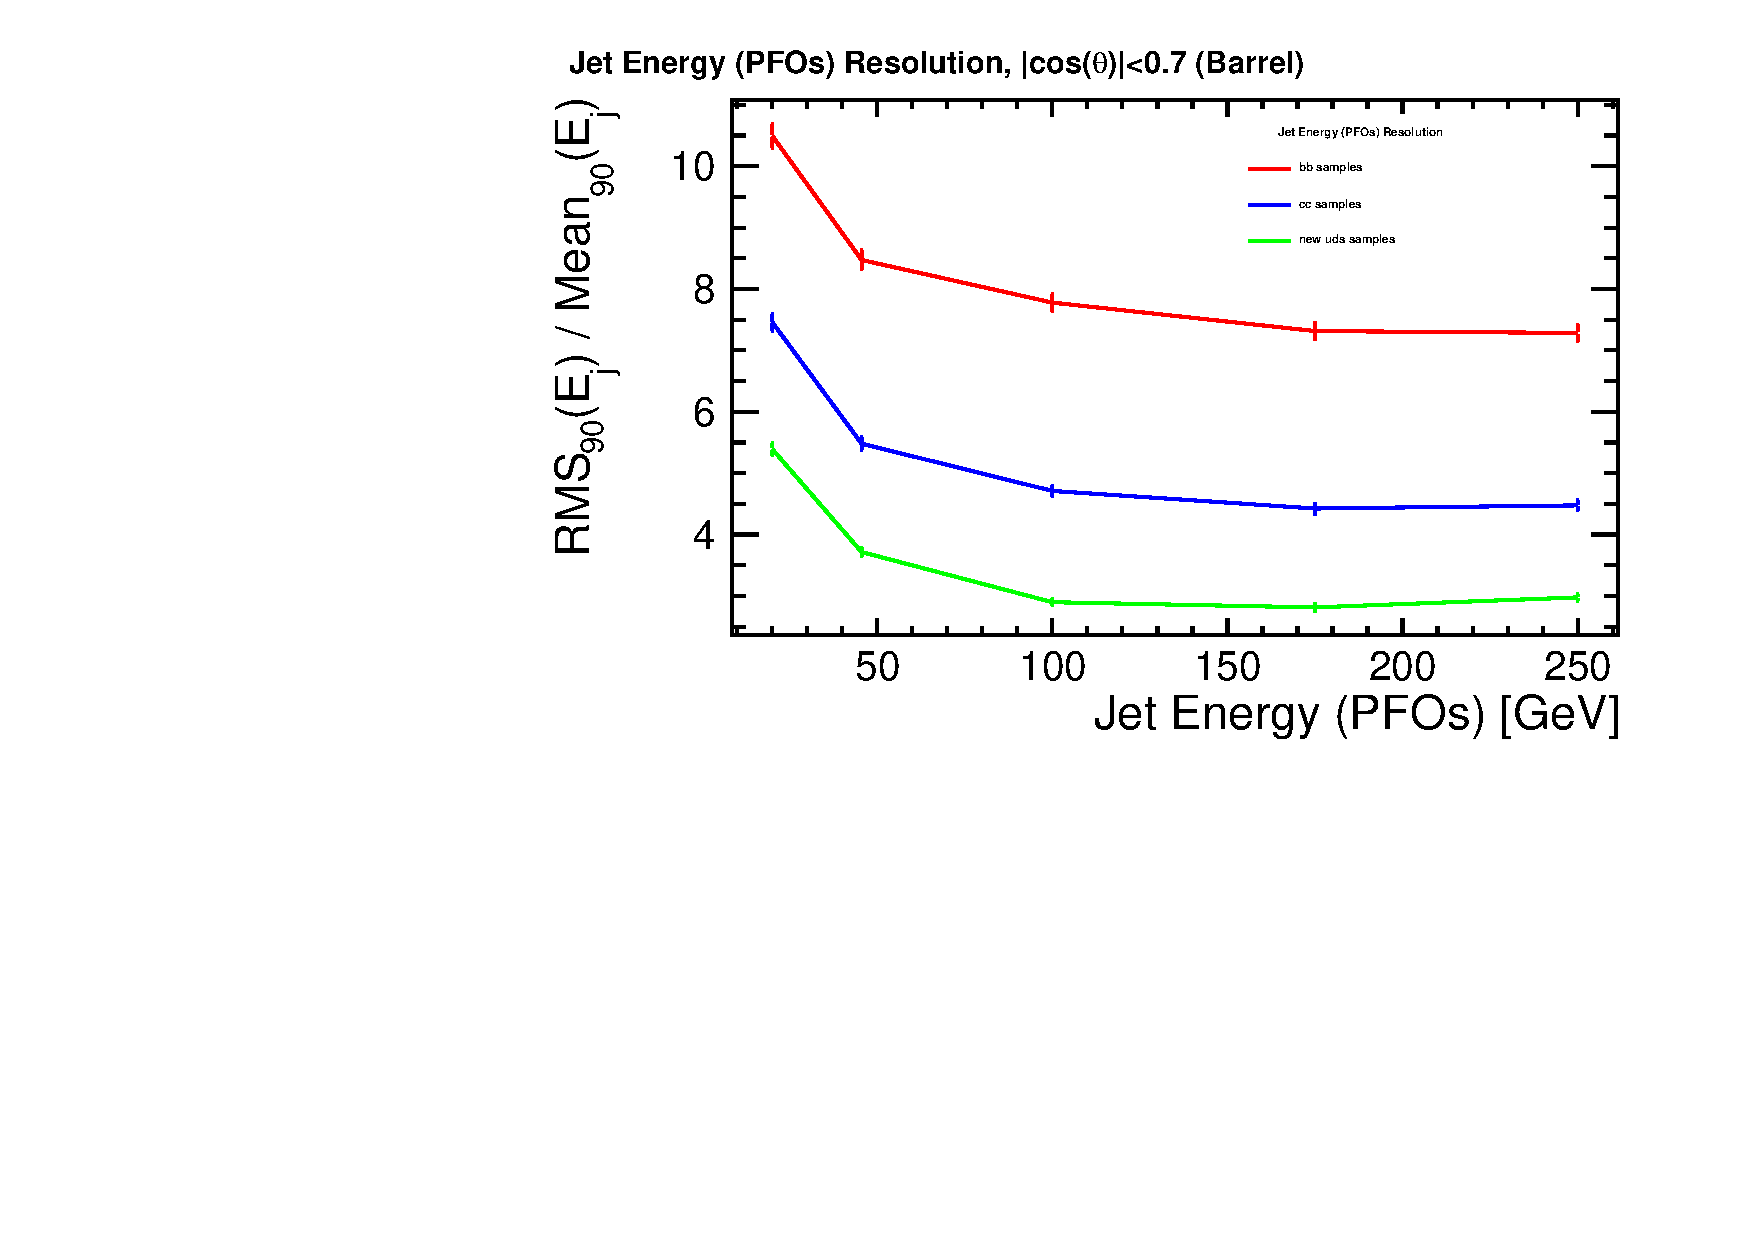
\includegraphics[width=0.5\hsize]{Performance/fig/Jet_Energy_Resolution_Barrel_rel_pfo_without_nu.pdf} &
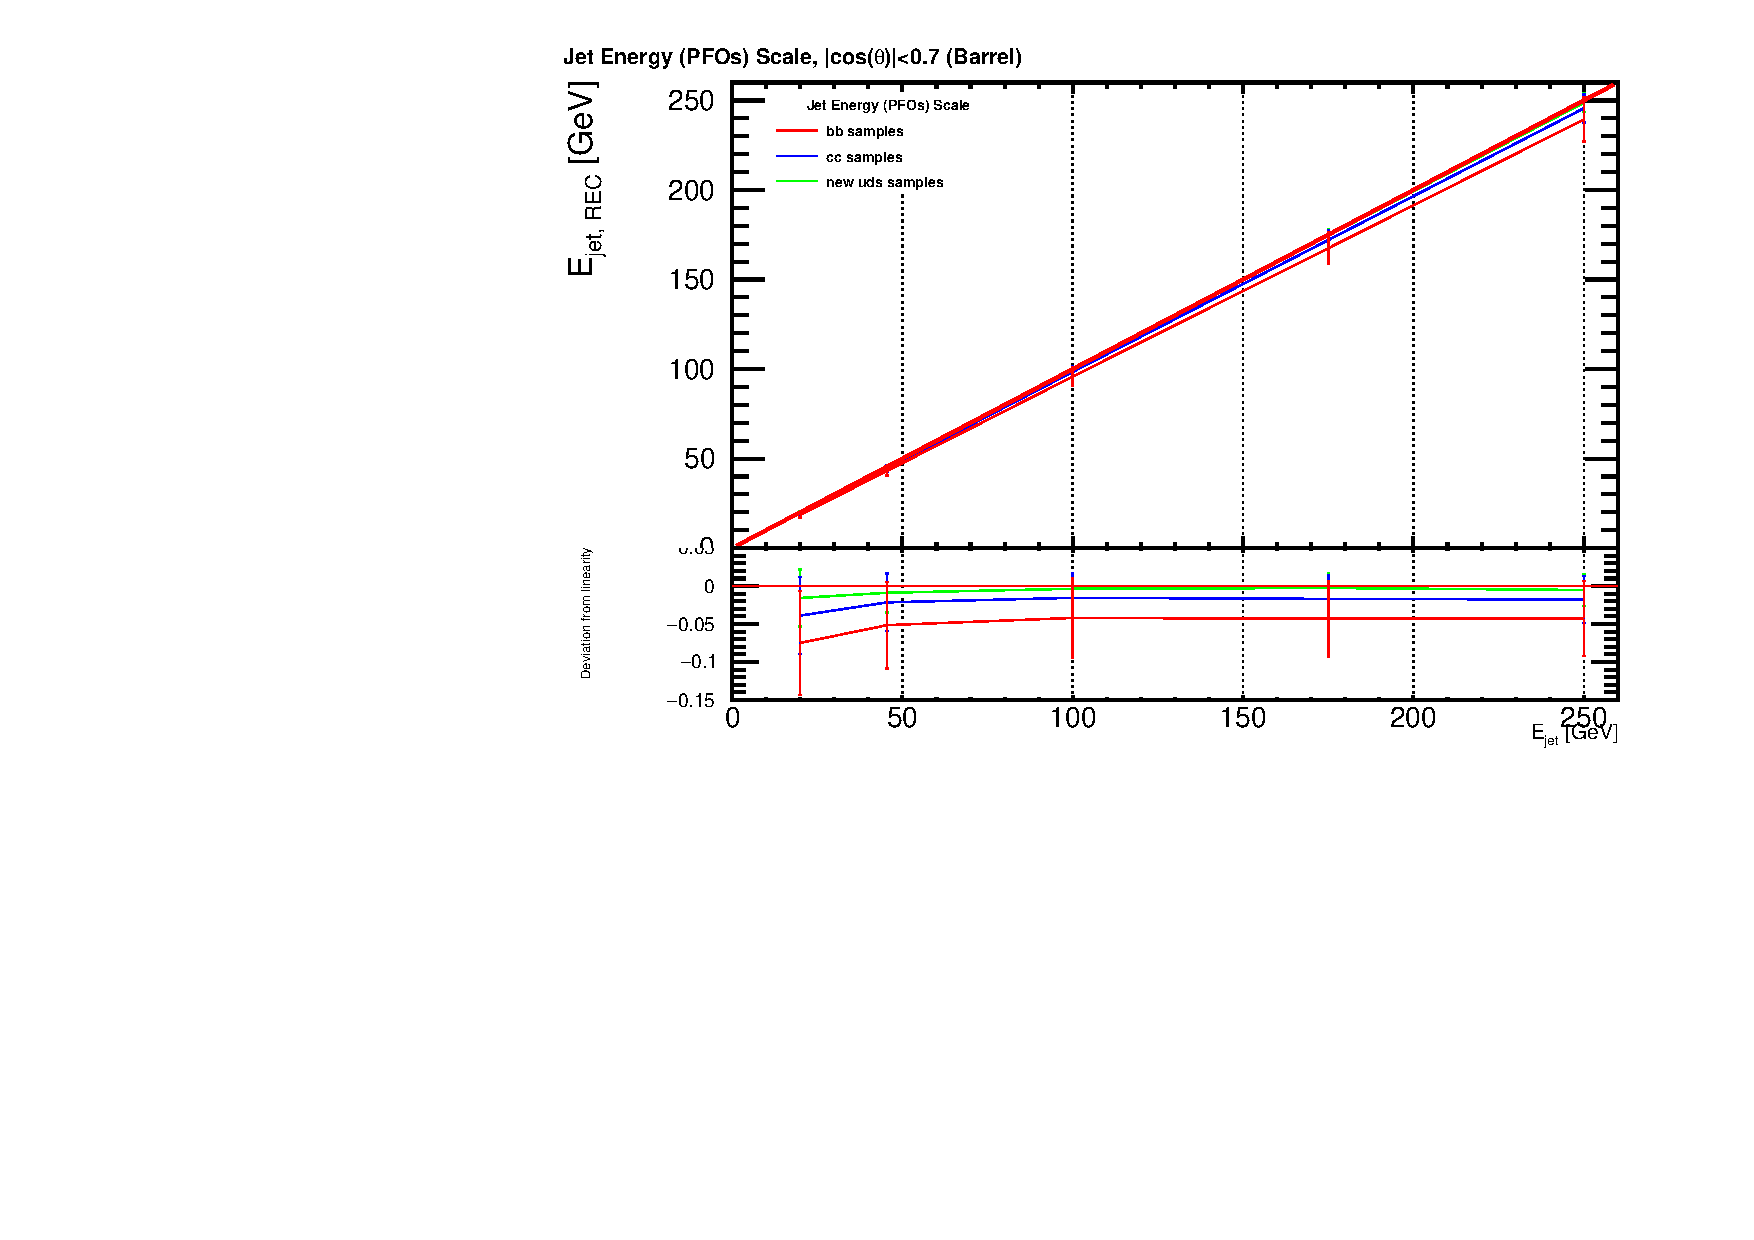
\includegraphics[width=0.5\hsize]{Performance/fig/Jet_Energy_Scale_Barrel_rel_pfo_without_nu.pdf}    \\
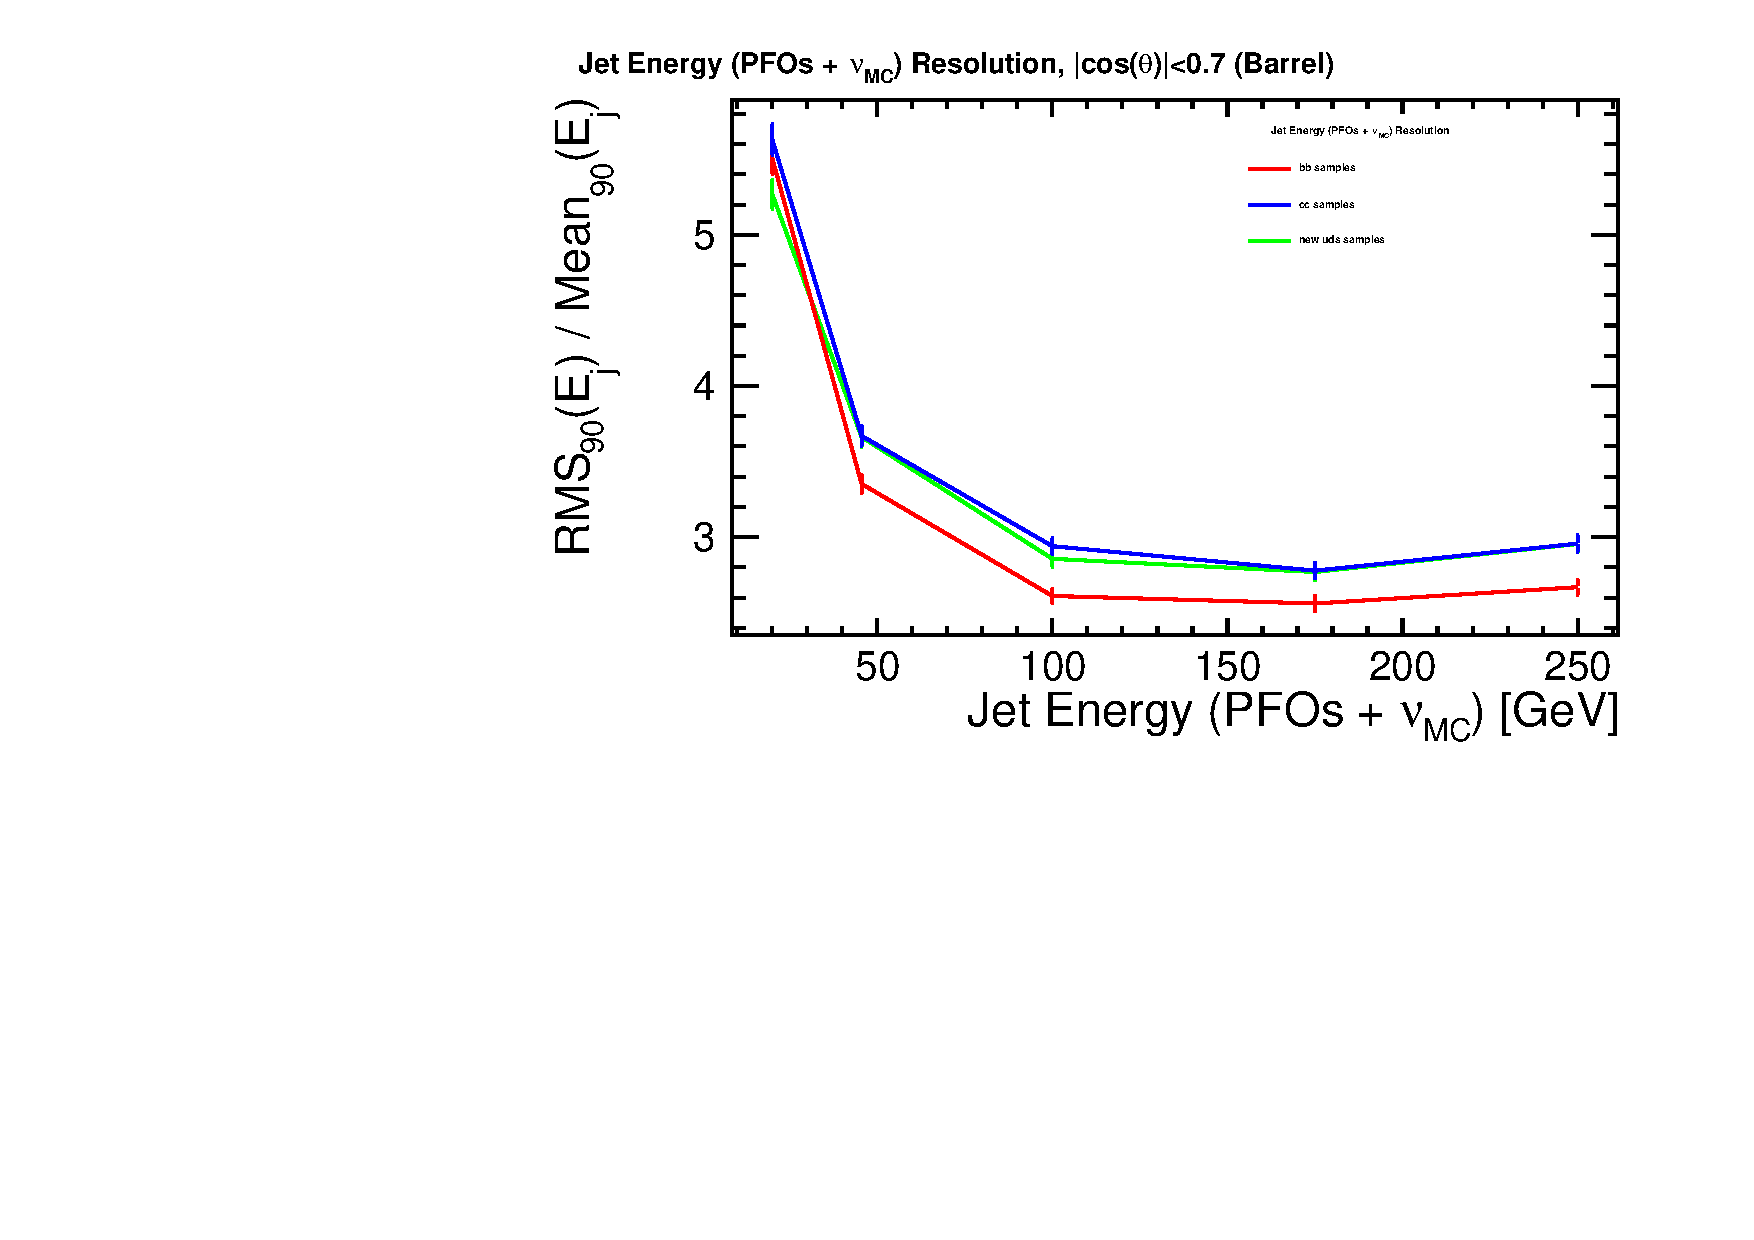
\includegraphics[width=0.5\hsize]{Performance/fig/Jet_Energy_Resolution_Barrel_rel_pfo_with_nu.pdf} &
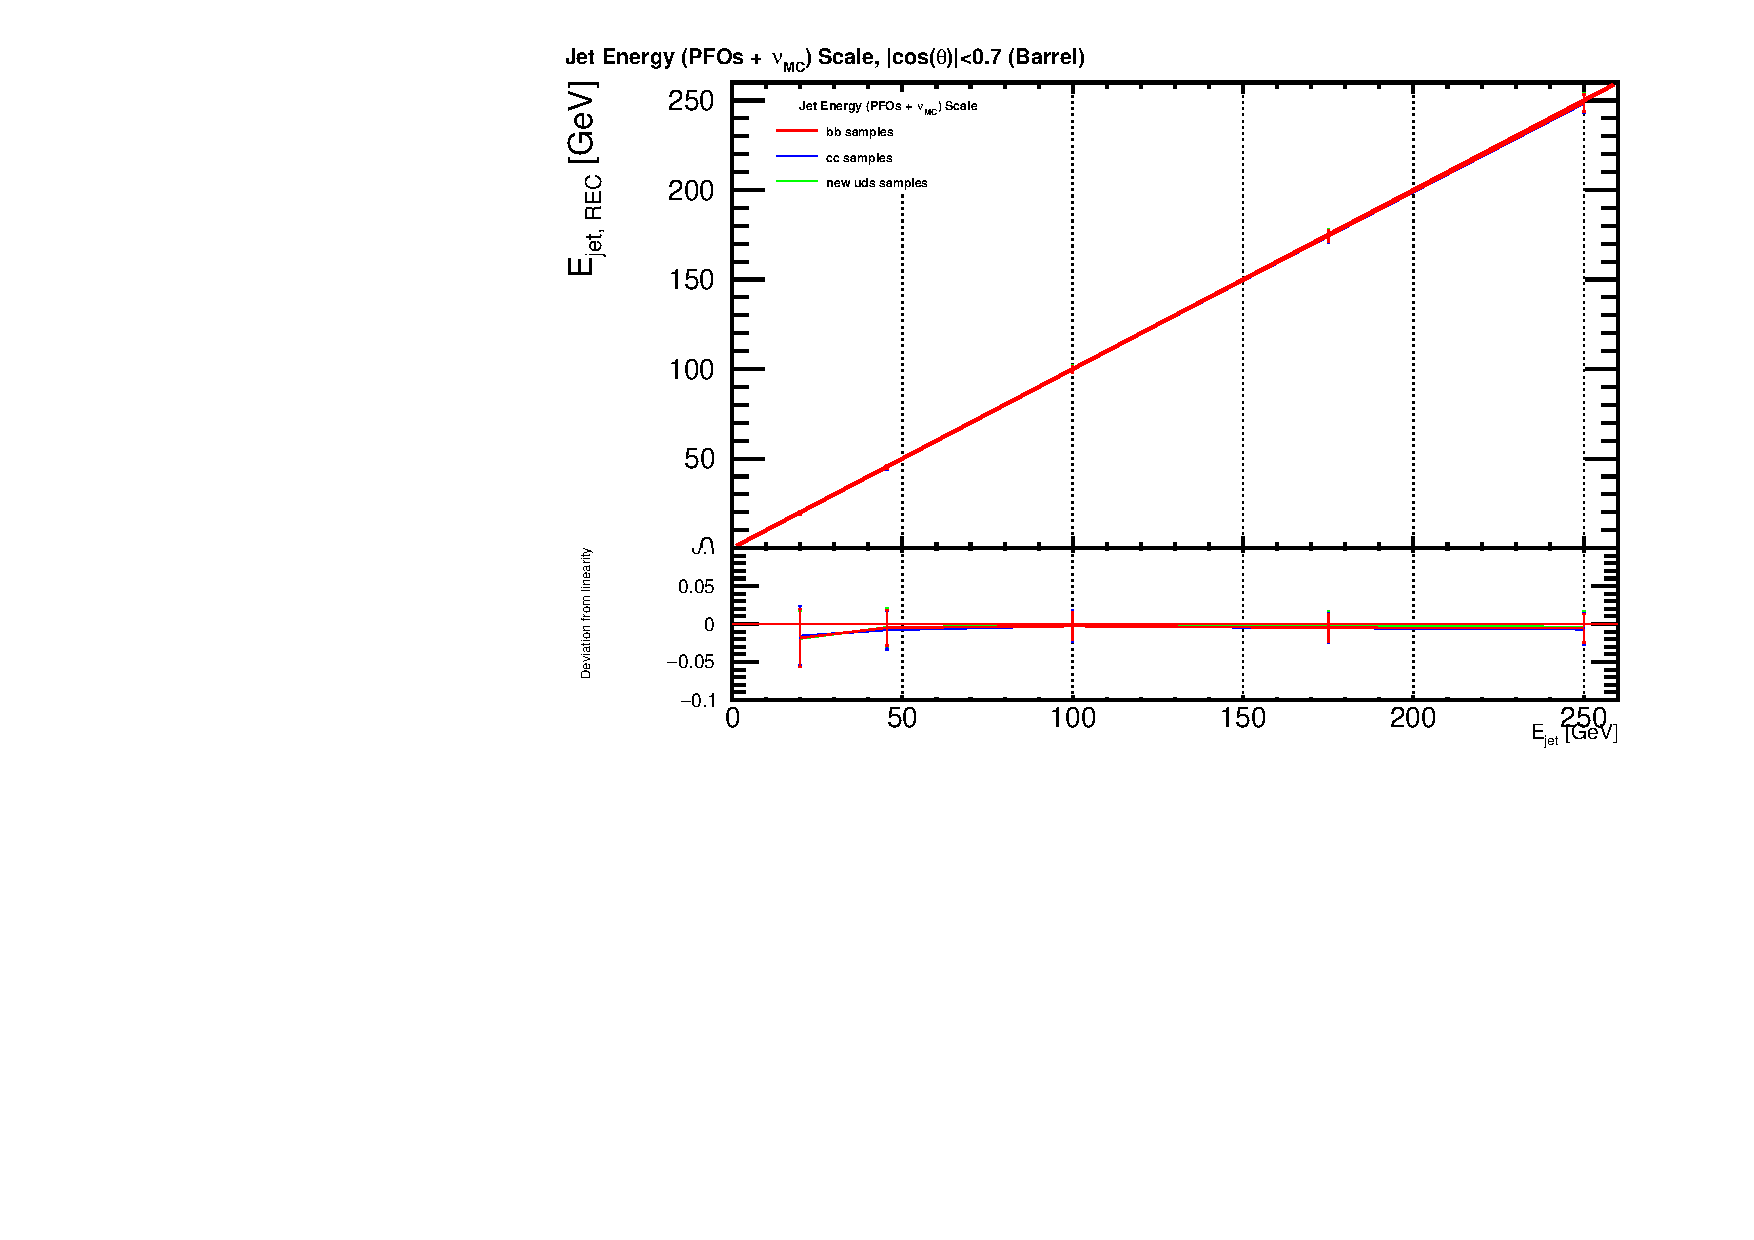
\includegraphics[width=0.5\hsize]{Performance/fig/Jet_Energy_Scale_Barrel_rel_pfo_with_nu.pdf}   
\end{tabular}
\caption{\label{fig:perf:trkeff_jer_ccbb} Jet energy resolution (left) and jet energy scale (right) for uds, cc and bb events as a function of the jet
  energy in the large ILD detecgtor model. Top row: without correction. Bottom row: with correcting the neutrino energy using the Monte-Carlo truth value. }
 \end{figure}


%%%%%%%%%%%%%%%%%%%%%%%%%%%%%%%%%%%%%%%%%%%%%%%%%%%%%%%%%%%%%%%
\subsection{Photon Reconstruction}

%%%%%%%%%%%%%%%%%%%%%%%%%%%%%%%%%%%%%%%%%%%%%%%%%%%%%%%%%%%%%%%
\subsection{Lepton ID}
\fix{muons, electrons}


%%%%%%%%%%%%%%%%%%%%%%%%%%%%%%%%%%%%%%%%%%%%%%%%%%%%%%%%%%%%%%%
\subsection{Charged Particle identification}

\fix{dE/dx, potentially ToF, shower shapes}

Figure~\ref{fig:perf:trkeff_jer_dedx} shows the separation power for $\pi/K$ and $K/p$  based on the $dE/dx$ measurement in the TPC (left) and the
possible improvement that could be achieved by combining it with a  {\em time-of-flight (TOF)} measurement (right). The TOF estimator used here is
computed using the first ten calorimeter hits in the Ecal that are closed to the extrapolation of the particles momentum into the calorimeter, assuming
an individual time resolution of $100$~ps per hit\footnote{While this time resolution seems realisticly possible, it has to be noted that so far it has
not yet been demonstrated in a test beam prototype.}.

%
% dE/dx separation power - combined w/ TOF
% 
\thisfloatsetup{floatwidth=\SfigwFull,capposition=beside}
\begin{figure}[b!]
\begin{tabular}{cc}
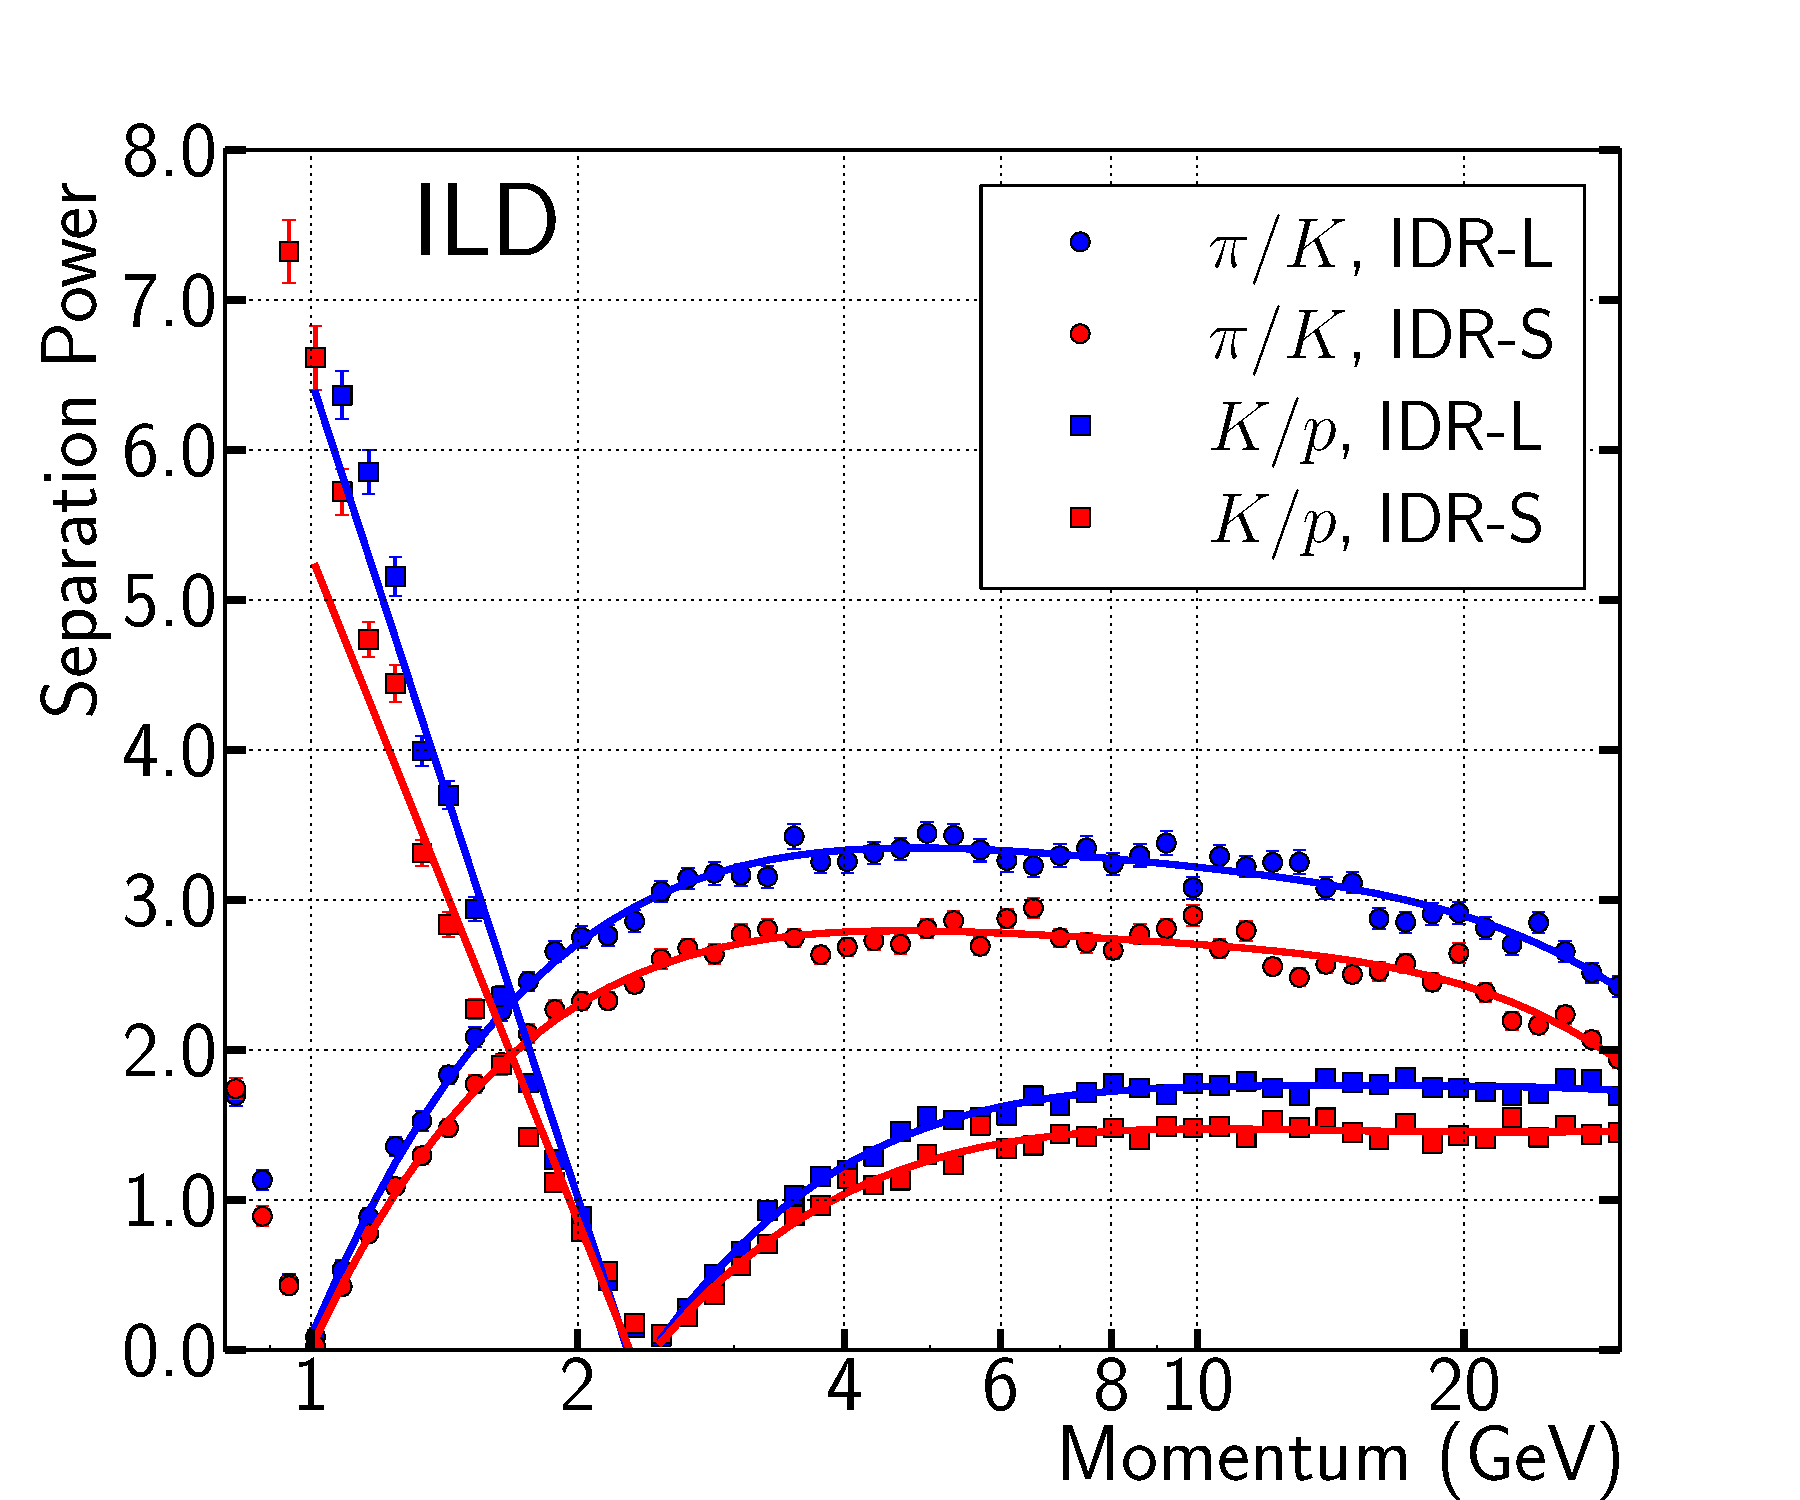
\includegraphics[width=0.5\hsize]{Performance/fig/dEdx_ILDls_separation_power.pdf} &
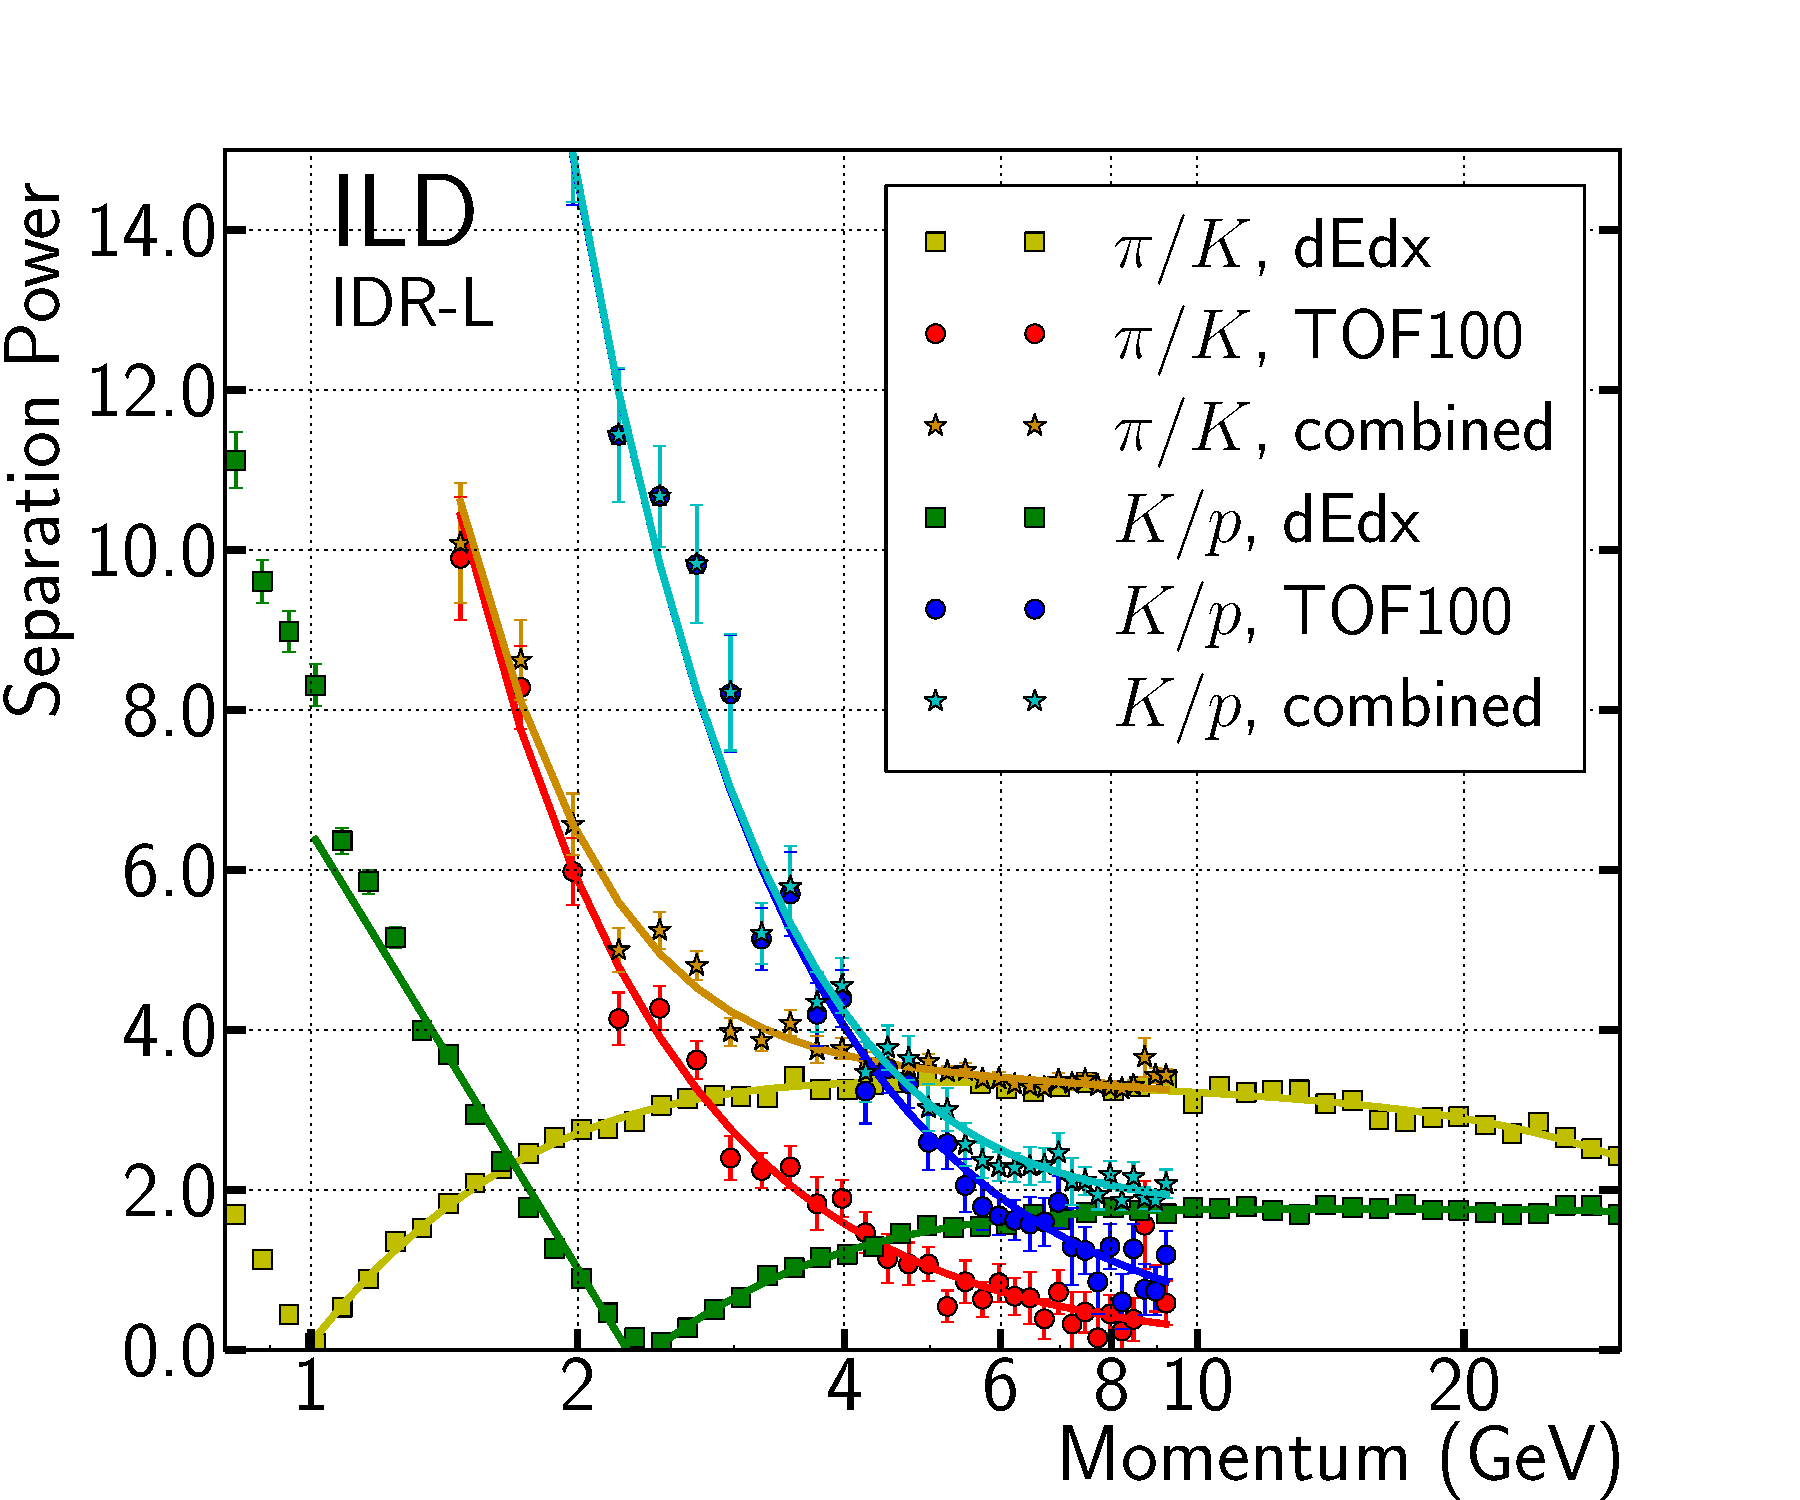
\includegraphics[width=0.5\hsize]{Performance/fig/Combined_dEdx_TOF100.pdf}
\end{tabular}
\caption{\label{fig:perf:trkeff_jer_dedx} Left: Particle separation power for $\pi/K$ and $K/p$ (left) based on the $dE/dx$ measurement in the TPC.
Right: improvement of the same separartion power if combined with a {\em time-of-flight (TOF)} estimator from the first ten Ecal layers.}
 \end{figure}

